% Auto-generated by experiments.analysis.generate_ci_plots --- do not edit.
\begin{figure}[H]
\centering
\adjustbox{max width=\textwidth}{%
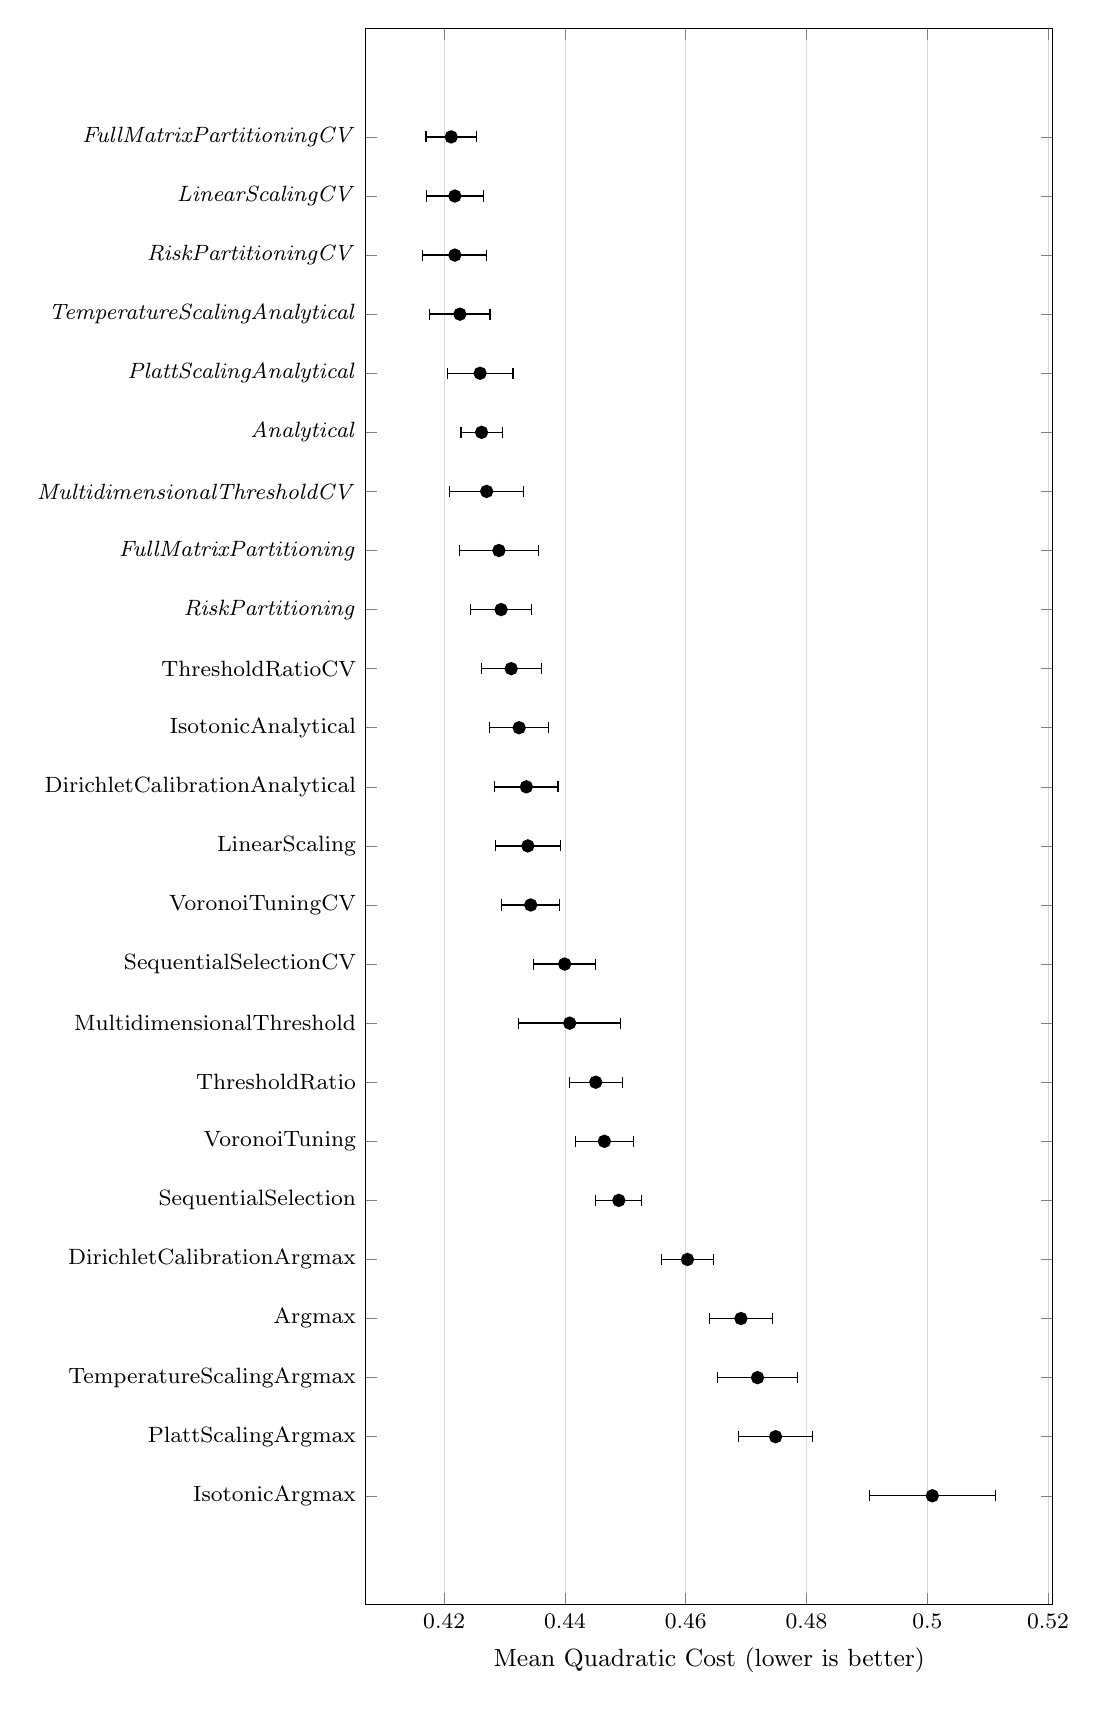
\begin{tikzpicture}
\begin{axis}[
    width=0.85\textwidth, height=21.60cm,
    xlabel={Mean Quadratic Cost (lower is better)},
    symbolic y coords={{FullMatrixPartitioningCV},{LinearScalingCV},{RiskPartitioningCV},{TemperatureScalingAnalytical},{PlattScalingAnalytical},{Analytical},{MultidimensionalThresholdCV},{FullMatrixPartitioning},{RiskPartitioning},{ThresholdRatioCV},{IsotonicAnalytical},{DirichletCalibrationAnalytical},{LinearScaling},{VoronoiTuningCV},{SequentialSelectionCV},{MultidimensionalThreshold},{ThresholdRatio},{VoronoiTuning},{SequentialSelection},{DirichletCalibrationArgmax},{Argmax},{TemperatureScalingArgmax},{PlattScalingArgmax},{IsotonicArgmax}},
    ytick={{FullMatrixPartitioningCV},{LinearScalingCV},{RiskPartitioningCV},{TemperatureScalingAnalytical},{PlattScalingAnalytical},{Analytical},{MultidimensionalThresholdCV},{FullMatrixPartitioning},{RiskPartitioning},{ThresholdRatioCV},{IsotonicAnalytical},{DirichletCalibrationAnalytical},{LinearScaling},{VoronoiTuningCV},{SequentialSelectionCV},{MultidimensionalThreshold},{ThresholdRatio},{VoronoiTuning},{SequentialSelection},{DirichletCalibrationArgmax},{Argmax},{TemperatureScalingArgmax},{PlattScalingArgmax},{IsotonicArgmax}},
    yticklabels={\textit{FullMatrixPartitioningCV},\textit{LinearScalingCV},\textit{RiskPartitioningCV},\textit{TemperatureScalingAnalytical},\textit{PlattScalingAnalytical},\textit{Analytical},\textit{MultidimensionalThresholdCV},\textit{FullMatrixPartitioning},\textit{RiskPartitioning},ThresholdRatioCV,IsotonicAnalytical,DirichletCalibrationAnalytical,LinearScaling,VoronoiTuningCV,SequentialSelectionCV,MultidimensionalThreshold,ThresholdRatio,VoronoiTuning,SequentialSelection,DirichletCalibrationArgmax,Argmax,TemperatureScalingArgmax,PlattScalingArgmax,IsotonicArgmax},
    y dir=reverse,
    enlarge y limits=0.08,
    xmajorgrids=true,
    major grid style={draw=black!15, line width=0.3pt},
    scaled x ticks=false,
    xticklabel style={/pgf/number format/fixed, /pgf/number format/precision=3},
    tick label style={font=\footnotesize},
    label style={font=\small},
    every axis plot/.append style={thick},
]
\addplot[only marks, mark=*, mark size=2pt, color=black, error bars/x dir=both, error bars/x explicit, error bars/error bar style={color=black, line width=0.5pt}] coordinates { (0.421172,{FullMatrixPartitioningCV}) +- (0.00416834,0) };
\addplot[only marks, mark=*, mark size=2pt, color=black, error bars/x dir=both, error bars/x explicit, error bars/error bar style={color=black, line width=0.5pt}] coordinates { (0.42177,{LinearScalingCV}) +- (0.00469818,0) };
\addplot[only marks, mark=*, mark size=2pt, color=black, error bars/x dir=both, error bars/x explicit, error bars/error bar style={color=black, line width=0.5pt}] coordinates { (0.42177,{RiskPartitioningCV}) +- (0.00528125,0) };
\addplot[only marks, mark=*, mark size=2pt, color=black, error bars/x dir=both, error bars/x explicit, error bars/error bar style={color=black, line width=0.5pt}] coordinates { (0.422608,{TemperatureScalingAnalytical}) +- (0.0049866,0) };
\addplot[only marks, mark=*, mark size=2pt, color=black, error bars/x dir=both, error bars/x explicit, error bars/error bar style={color=black, line width=0.5pt}] coordinates { (0.425957,{PlattScalingAnalytical}) +- (0.00544211,0) };
\addplot[only marks, mark=*, mark size=2pt, color=black, error bars/x dir=both, error bars/x explicit, error bars/error bar style={color=black, line width=0.5pt}] coordinates { (0.426196,{Analytical}) +- (0.00340226,0) };
\addplot[only marks, mark=*, mark size=2pt, color=black, error bars/x dir=both, error bars/x explicit, error bars/error bar style={color=black, line width=0.5pt}] coordinates { (0.427033,{MultidimensionalThresholdCV}) +- (0.00608365,0) };
\addplot[only marks, mark=*, mark size=2pt, color=black, error bars/x dir=both, error bars/x explicit, error bars/error bar style={color=black, line width=0.5pt}] coordinates { (0.429067,{FullMatrixPartitioning}) +- (0.00654211,0) };
\addplot[only marks, mark=*, mark size=2pt, color=black, error bars/x dir=both, error bars/x explicit, error bars/error bar style={color=black, line width=0.5pt}] coordinates { (0.429426,{RiskPartitioning}) +- (0.00501822,0) };
\addplot[only marks, mark=*, mark size=2pt, color=black, error bars/x dir=both, error bars/x explicit, error bars/error bar style={color=black, line width=0.5pt}] coordinates { (0.4311,{ThresholdRatioCV}) +- (0.0049551,0) };
\addplot[only marks, mark=*, mark size=2pt, color=black, error bars/x dir=both, error bars/x explicit, error bars/error bar style={color=black, line width=0.5pt}] coordinates { (0.432416,{IsotonicAnalytical}) +- (0.00489392,0) };
\addplot[only marks, mark=*, mark size=2pt, color=black, error bars/x dir=both, error bars/x explicit, error bars/error bar style={color=black, line width=0.5pt}] coordinates { (0.433612,{DirichletCalibrationAnalytical}) +- (0.00524818,0) };
\addplot[only marks, mark=*, mark size=2pt, color=black, error bars/x dir=both, error bars/x explicit, error bars/error bar style={color=black, line width=0.5pt}] coordinates { (0.433852,{LinearScaling}) +- (0.00535553,0) };
\addplot[only marks, mark=*, mark size=2pt, color=black, error bars/x dir=both, error bars/x explicit, error bars/error bar style={color=black, line width=0.5pt}] coordinates { (0.43433,{VoronoiTuningCV}) +- (0.00476955,0) };
\addplot[only marks, mark=*, mark size=2pt, color=black, error bars/x dir=both, error bars/x explicit, error bars/error bar style={color=black, line width=0.5pt}] coordinates { (0.439952,{SequentialSelectionCV}) +- (0.00509619,0) };
\addplot[only marks, mark=*, mark size=2pt, color=black, error bars/x dir=both, error bars/x explicit, error bars/error bar style={color=black, line width=0.5pt}] coordinates { (0.440789,{MultidimensionalThreshold}) +- (0.00843233,0) };
\addplot[only marks, mark=*, mark size=2pt, color=black, error bars/x dir=both, error bars/x explicit, error bars/error bar style={color=black, line width=0.5pt}] coordinates { (0.445096,{ThresholdRatio}) +- (0.00438397,0) };
\addplot[only marks, mark=*, mark size=2pt, color=black, error bars/x dir=both, error bars/x explicit, error bars/error bar style={color=black, line width=0.5pt}] coordinates { (0.446531,{VoronoiTuning}) +- (0.00475151,0) };
\addplot[only marks, mark=*, mark size=2pt, color=black, error bars/x dir=both, error bars/x explicit, error bars/error bar style={color=black, line width=0.5pt}] coordinates { (0.448923,{SequentialSelection}) +- (0.00380797,0) };
\addplot[only marks, mark=*, mark size=2pt, color=black, error bars/x dir=both, error bars/x explicit, error bars/error bar style={color=black, line width=0.5pt}] coordinates { (0.460287,{DirichletCalibrationArgmax}) +- (0.00435614,0) };
\addplot[only marks, mark=*, mark size=2pt, color=black, error bars/x dir=both, error bars/x explicit, error bars/error bar style={color=black, line width=0.5pt}] coordinates { (0.469139,{Argmax}) +- (0.00524985,0) };
\addplot[only marks, mark=*, mark size=2pt, color=black, error bars/x dir=both, error bars/x explicit, error bars/error bar style={color=black, line width=0.5pt}] coordinates { (0.47189,{TemperatureScalingArgmax}) +- (0.0066175,0) };
\addplot[only marks, mark=*, mark size=2pt, color=black, error bars/x dir=both, error bars/x explicit, error bars/error bar style={color=black, line width=0.5pt}] coordinates { (0.47488,{PlattScalingArgmax}) +- (0.00615896,0) };
\addplot[only marks, mark=*, mark size=2pt, color=black, error bars/x dir=both, error bars/x explicit, error bars/error bar style={color=black, line width=0.5pt}] coordinates { (0.500837,{IsotonicArgmax}) +- (0.0104509,0) };
\end{axis}
\end{tikzpicture}%
}
\caption{abalone: Quadratic Cost on LGBM (lower is better). Each dot is a strategy's mean over ten seeds with a $\pm 1$ SE horizontal bar; rows are sorted by mean, and the best strategy and any whose interval overlaps it are italicized.}%
\label{fig:ci-abalone-quadratic_cost}
\end{figure}
